% =================================================================================================
% File:			server_tier/miner.tex
% Description:	Definisce la sezione relativa al back-end dell'applicazione
% Created:		2015-04-07
% Author:		Cusinato Giacomo
% Email:		cusinato.giacomo@mashup-unipd.it
% =================================================================================================
% Modification History:
% Version		Modifier Date		Change											Author
% 0.0.1
% 0.0.2			2015-05-21			Inserim. descrizione attributi e sist. grafici	Luca Santacatterina
% =================================================================================================

% CONTENUTO DEL CAPITOLO


\subsubsection{server::miner} % (fold)
\label{ssub:bdsm_app_server_miner}
\begin{figure}[htbp]
	\centering
	\centerline{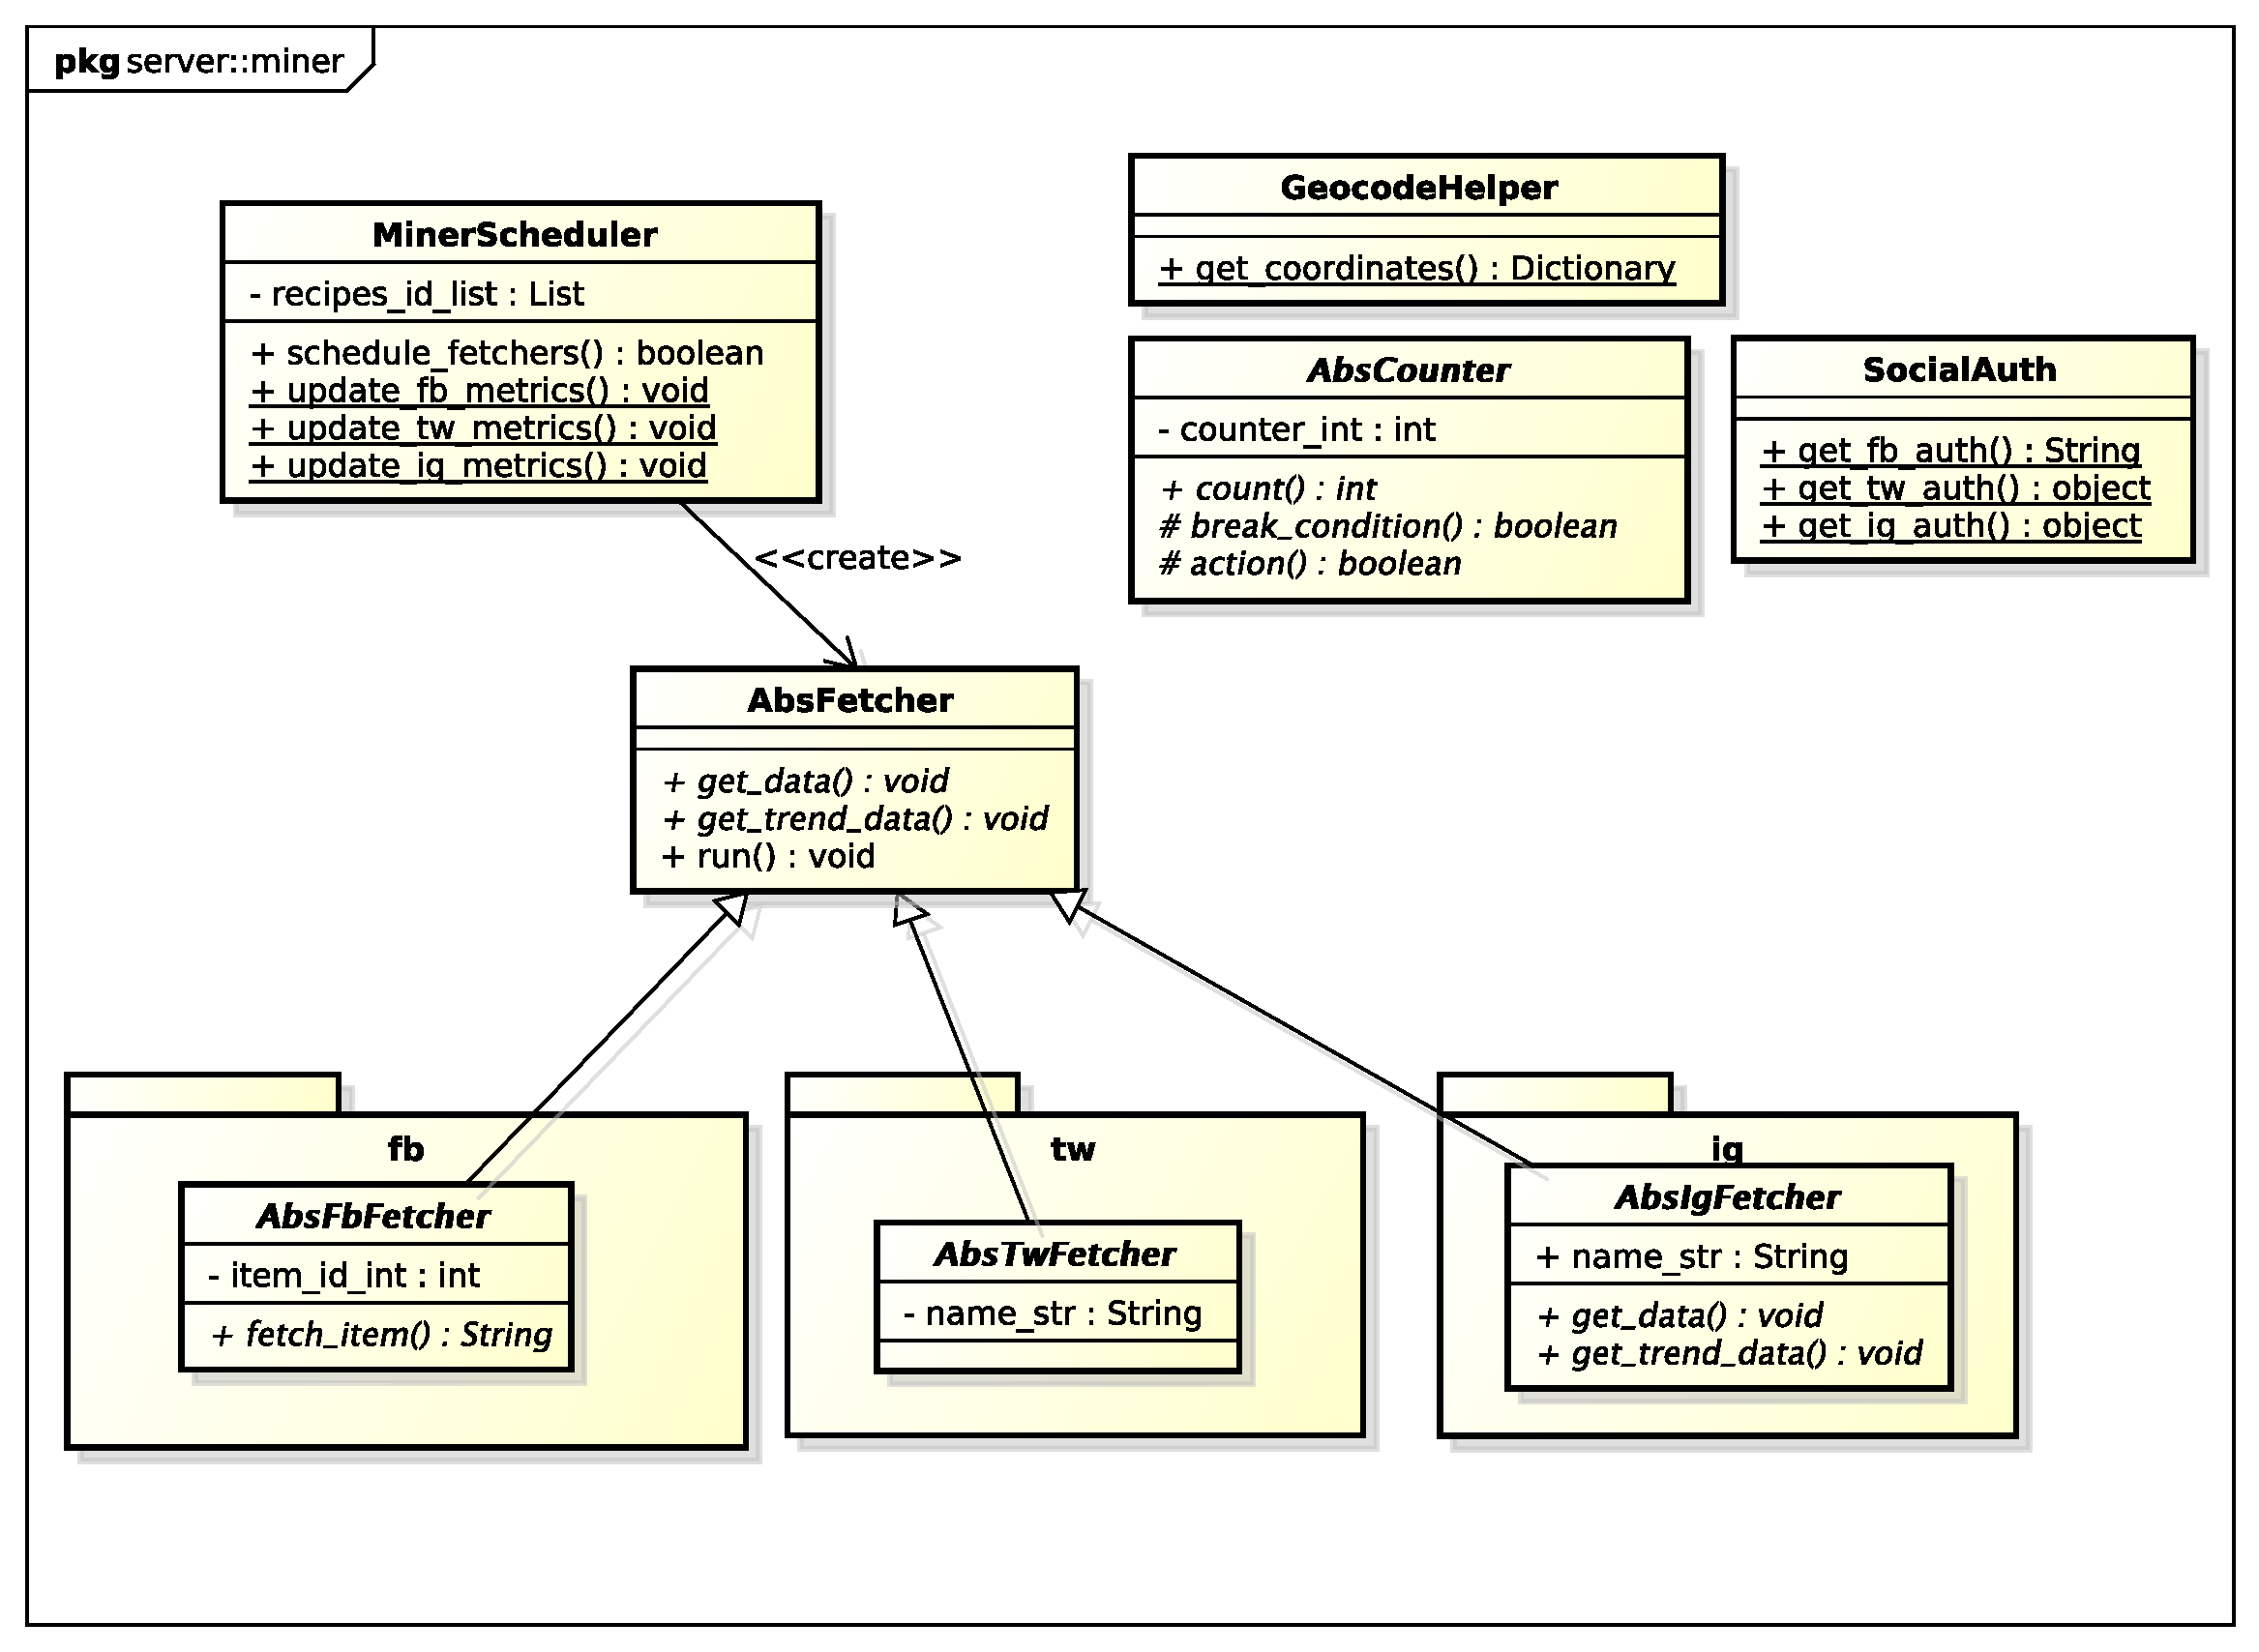
\includegraphics[scale=0.4]{./images/server/miner.pdf}}
	\caption{Package - server::miner}
\end{figure}

\begin{itemize}
  \item \textbf{Descrizione}: è il package che contiene tutte le classi che includono i metodi per prelevare i dati grezzi dai vari social network e salvarli nel database;
  \item \textbf{Padre}: server
  \item \textbf{Package contenuti}:
  	\begin{itemize}
  		\item server::miner::fb
  		\item server::miner::ig
  		\item server::miner::tw
  	\end{itemize}
  \item \textbf{Interazione con altri componenti}:
  	\begin{itemize}
  		\item server::processor
  		\item server::db
  	\end{itemize}
\end{itemize}

\paragraph{Classi} % (fold)
		\subparagraph{server::miner::MinerScheduler} % (fold)
		\label{subp:server_miner_MinerScheduler}
			\begin{itemize}
				\item \textbf{Descrizione}: classe che si occupa di creare i fetcher che preleveranno i dati per ogni metrica di ogni social network;
				\item \textbf{Utilizzo}: contiene la lista degli id delle Recipe da aggiornare ed un metodo che inizializza e avvia i vari fetcher;
				\item \textbf{Relazioni con altre classi}:
					\begin{itemize}
						\item server::miner::AbsFetcher
					\end{itemize}
				\item \textbf{Attributi}:
					\begin{itemize}
						\item \textcolor{forestgreen}{\texttt{recipes\_id\_list : List}}
						\begin{description}
							\item \textbf{Descrizione}: lista di recipes da aggiornare;
						\end{description}
					\end{itemize}
				\item \textbf{Metodi}:   
					\begin{itemize}
						\item \textcolor{forestgreen}{\texttt{+ \_\_init\_\_(recipe\_id\_list : int ) : void}}
						\begin{description}
							\item \textbf{Descrizione}: costruttore della classe di default. Inizializza la variabile recipe\_id\_list con la lista delle ricette da aggiornare;
						\end{description}
						\item \textcolor{forestgreen}{\texttt{+ schedule\_fetchers() : void}}
						\begin{description}
							\item \textbf{Descrizione}: avvia l'update delle recipes contenute nella lista passata;
						\end{description}
						\item \textcolor{forestgreen}{\texttt{+ update\_fb\_metrics(recipe\_id : String) : void}}
						\begin{description}
							\item \textbf{Descrizione}: il metodo controlla il tipo di recipe e avvia l'aggiornamento della recipe di Facebook;
						\end{description}
						\item \textcolor{forestgreen}{\texttt{+ update\_ig\_metrics(recipe\_id : String) : void}}
						\begin{description}
							\item \textbf{Descrizione}: il metodo controlla il tipo di recipe e avvia l'aggiornamento della recipe di Instagram;
						\end{description}
						\item \textcolor{forestgreen}{\texttt{+ update\_tw\_metrics(recipe\_id : String) : void}}
						\begin{description}
							\item \textbf{Descrizione}: il metodo controlla il tipo di recipe e avvia l'aggiornamento della recipe di Twitter;
						\end{description}
					\end{itemize}
			\end{itemize}
		% subparagraph server_miner_MinerScheduler [end]

		\subparagraph{server::miner::AbsCounter} % (fold)
		\label{subp:server_miner_AbsCounter}
			\begin{itemize}
				\item \textbf{Descrizione}: classe astratta che rappresenta il padre delle classi counter delle varie metriche;
				\item \textbf{Utilizzo}: descrive lo scheletro dell'algoritmo di counting necessario ad effettuare il conteggio di determinati dati ricavati con lo scopo ottenere un trend;
				\item \textbf{Relazioni con altre classi}:
					\begin{itemize}
						\item server::miner::fb::AbsFbCounter
						\item server::miner::tw::AbsTwCounter
						\item server::miner::ig::AbsIgCounter
					\end{itemize}
				\item \textbf{Attributi}: 
					\begin{itemize}
						\item \textcolor{forestgreen}{\texttt{counter\_int : int}}
						\begin{description}
							\item \textbf{Descrizione}: contiene la somma richiesta;
						\end{description}
					\end{itemize}
				\item \textbf{Metodi}:   
					\begin{itemize}
						\item \textcolor{forestgreen}{\texttt{+ \_\_init\_\_() : void}}
						\begin{description}
							\item \textbf{Descrizione}: costruttore della classe di default. Inizializza la variabile del contatore a 0;
						\end{description}
						\item \textcolor{forestgreen}{\texttt{+ abstract action() : void}}
						\begin{description}
							\item \textbf{Descrizione}: il metodo in questa classe viene solamente marcato come astratto, verrà implementato successivamente nelle classi figlie. Il metodo viene utilizzato in ogni elemento ciclato;
						\end{description}
						\item \textcolor{forestgreen}{\texttt{+ abstract break\_condition() : void}}
						\begin{description}
							\item \textbf{Descrizione}: il metodo in questa classe viene solamente marcato come astratto, verrà implementato successivamente nelle classi figlie. Il metodo blocca il count degli elementi;
						\end{description}
						\item \textcolor{forestgreen}{\texttt{+ abstract count() : void}}
						\begin{description}
							\item \textbf{Descrizione}: il metodo in questa classe viene solamente marcato come astratto, verrà implementato successivamente nelle classi figlie. Il metodo avvia il count degli elementi ;
						\end{description}
					\end{itemize}
			\end{itemize}
		% subparagraph server_miner_AbsCounter [end]

		\subparagraph{server::miner::AbsFetcher} % (fold)
		\label{subp:server_miner_AbsFetcher}
				\begin{itemize}
				\item \textbf{Descrizione}: classe astratta che rappresenta il padre delle classi fetcher dei vari social network;
				\item \textbf{Utilizzo}: è utilizzata per mantenere l'estensibilità nel caso l'applicazione venga estesa con altre API  oltre a quelli dei social network presi in considerazione;
				\item \textbf{Relazioni con altre classi}:
					\begin{itemize}
						\item server::miner::fb::AbsFbFetcher
						\item server::miner::tw::AbsTwFetcher
						\item server::miner::ig::AbsIgFetcher
					\end{itemize}
				\item \textbf{Attributi}: N/A
				\item \textbf{Metodi}:
					\begin{itemize}
						\item \textcolor{forestgreen}{\texttt{+ abstract get\_data() : void}}
						\begin{description}
							\item \textbf{Descrizione}: il metodo in questa classe viene solamente marcato come astratto, verrà implementato successivamente nelle classi figlie. Il metodo ottiene i dati statici del post;
						\end{description}
						\item \textcolor{forestgreen}{\texttt{+ abstract get\_trend\_data() : void}}
						\begin{description}
							\item \textbf{Descrizione}: il metodo in questa classe viene solamente marcato come astratto, verrà implementato successivamente nelle classi figlie. Il metodo ottiene i dati del trend;
						\end{description}
						\item \textcolor{forestgreen}{\texttt{+ run() : void}}
						\begin{description}
							\item \textbf{Descrizione}: il metodo avvia sequenzialmente get\_data ed get\_trend\_data;
						\end{description}
					\end{itemize}
			\end{itemize}
		% subparagraph server_miner_AbsFetcher [end]

		\subparagraph{server::miner::SocialAuth} % (fold)
		\label{subp:server_miner_SocialAuth}
				\begin{itemize}
				\item \textbf{Descrizione}: classe che rappresenta la fase di autenticazione dei social network;
				\item \textbf{Utilizzo}: fornisce metodi statici per effettuare l'autenticazione ai social network presi in considerazione;
				\item \textbf{Relazioni con altre classi}:
					\begin{itemize}
						\item server::miner::fb::FbEventFetcher
						\item server::miner::fb::FbPageFetcher
						\item server::miner::fb::PostsCounter
						\item server::miner::tw::TwHashtagFetcher
						\item server::miner::tw::HashtagTweetCounter
						\item server::miner::tw::TwUserFetcher
						\item server::miner::tw::UserTweetCounter
						\item server::miner::ig::IgUserFetcher
						\item server::miner::ig::IgHastagFetcher
						\item server::miner::ig::MediaCounter
					\end{itemize}
				\item \textbf{Attributi}:
					\begin{itemize}
						\item \textcolor{forestgreen}{\texttt{- \_\_FACEBOOK\_APP\_ID : int}}
						\begin{description}
							\item \textbf{Descrizione}: la variabile deve essere definita costante e privata. Contiene l'id di autenticazione di Facebook;
						\end{description}
						\item \textcolor{forestgreen}{\texttt{- \_\_FACEBOOK\_APP\_SECRET : int}}
						\begin{description}
							\item \textbf{Descrizione}: la variabile deve essere definita costante e privata. Contiene l'id di autenticazione di Facebook;
						\end{description}
						\item \textcolor{forestgreen}{\texttt{- \_\_CONSUMER\_KEY : int}}
						\begin{description}
							\item \textbf{Descrizione}: la variabile deve essere definita costante e privata. Contiene l'access token utente pubblico di autenticazione di Twitter;
						\end{description}
						\item \textcolor{forestgreen}{\texttt{- \_\_CONSUMER\_SECRET : int}}
						\begin{description}
							\item \textbf{Descrizione}: la variabile deve essere definita costante e privata. Contiene l'access token utente privato di autenticazione di Twitter;
						\end{description}
						\item \textcolor{forestgreen}{\texttt{- \_\_ACCESS\_TOKEN : int}}
						\begin{description}
							\item \textbf{Descrizione}: la variabile deve essere definita costante e privata. Contiene l'access token pubblico di autenticazione di Twitter;
						\end{description}
						\item \textcolor{forestgreen}{\texttt{- \_\_ACCESS\_TOKEN\_SECRET : int}}
						\begin{description}
							\item \textbf{Descrizione}: la variabile deve essere definita costante e privata. Contiene l'access token privato di autenticazione di Twitter;
						\end{description}
						\item \textcolor{forestgreen}{\texttt{- \_\_CLIENT\_ID : int}}
						\begin{description}
							\item \textbf{Descrizione}: la variabile deve essere definita costante e privata. Contiene il client id pubblico di autenticazione di Instagram;
						\end{description}
						\item \textcolor{forestgreen}{\texttt{- \_\_CLIENT\_SECRET : int}}
						\begin{description}
							\item \textbf{Descrizione}: la variabile deve essere definita costante e privata. Contiene il client id privato di autenticazione di Instagram;
						\end{description}
						\item \textcolor{forestgreen}{\texttt{- \_\_ACCESS\_TOKEN : int}}
						\begin{description}
							\item \textbf{Descrizione}: la variabile deve essere definita costante e privata. Contiene l'access token di autenticazione di Instagram;
						\end{description}
					\end{itemize}
				\item \textbf{Metodi}:
					\begin{itemize}
						\item \textcolor{forestgreen}{\texttt{+ static get\_fb\_auth() : String}}
						\begin{description}
							\item \textbf{Descrizione}: il metodo deve essere dichiarato statico. Il metodo ha il compito di effettuare l'autenticazione su Facebook e di restituire l'access token valido per le chiamate;
						\end{description}
						\item \textcolor{forestgreen}{\texttt{+ static get\_tw\_auth() : String}}
						\begin{description}
							\item \textbf{Descrizione}: il metodo deve essere dichiarato statico. Il metodo ha il compito di effettuare l'autenticazione su Twitter e di restituire l'access token valido per le chiamate;
						\end{description}
						\item \textcolor{forestgreen}{\texttt{+ static get\_ig\_auth() : String}}
						\begin{description}
							\item \textbf{Descrizione}: il metodo deve essere dichiarato statico. Il metodo ha il compito di effettuare l'autenticazione su Instagram e di restituire il l'access token valido per le chiamate;
						\end{description}
					\end{itemize}
			\end{itemize}
		% subparagraph server_miner_SocialAuth [end]

		\subparagraph{server::miner::GeocodeHelper} % (fold)
		\label{subp:server_miner_GeocodeHelper}
				\begin{itemize}
				\item \textbf{Descrizione}: classe che si occupa di convertire la geolocalizzazione;
				\item \textbf{Utilizzo}: fornisce metodi statici ai social network presi in considerazione per la conversione dei luoghi in latitudine e longitudine;
				\item \textbf{Relazioni con altre classi}:
					\begin{itemize}
						\item server::miner::fb::FbEventFetcher
						\item server::miner::tw::UserTweetCounter
						\item server::miner::ig::MediaCounter
					\end{itemize}
				\item \textbf{Attributi}: N/A
				\item \textbf{Metodi}:
					\begin{itemize}
						\item \textcolor{forestgreen}{\texttt{+ static get\_coordinates(location\_str : String) : Dictionary}}
						\begin{description}
							\item \textbf{Descrizione}: il metodo deve essere dichiarato statico. Il metodo ha il compito di ricevere un indirizzo o una città e restituire le relative coordinate di latitudine e longitudine sottoforma di dizionario;
						\end{description}
					\end{itemize}
			\end{itemize}
		% subparagraph server_miner_GeocodeHelper [end]

\subsubsection{server::miner::fb} % (fold)
\label{ssub:bdsm_app_server_miner_fb}
\begin{figure}[htbp]
	\centering
	\centerline{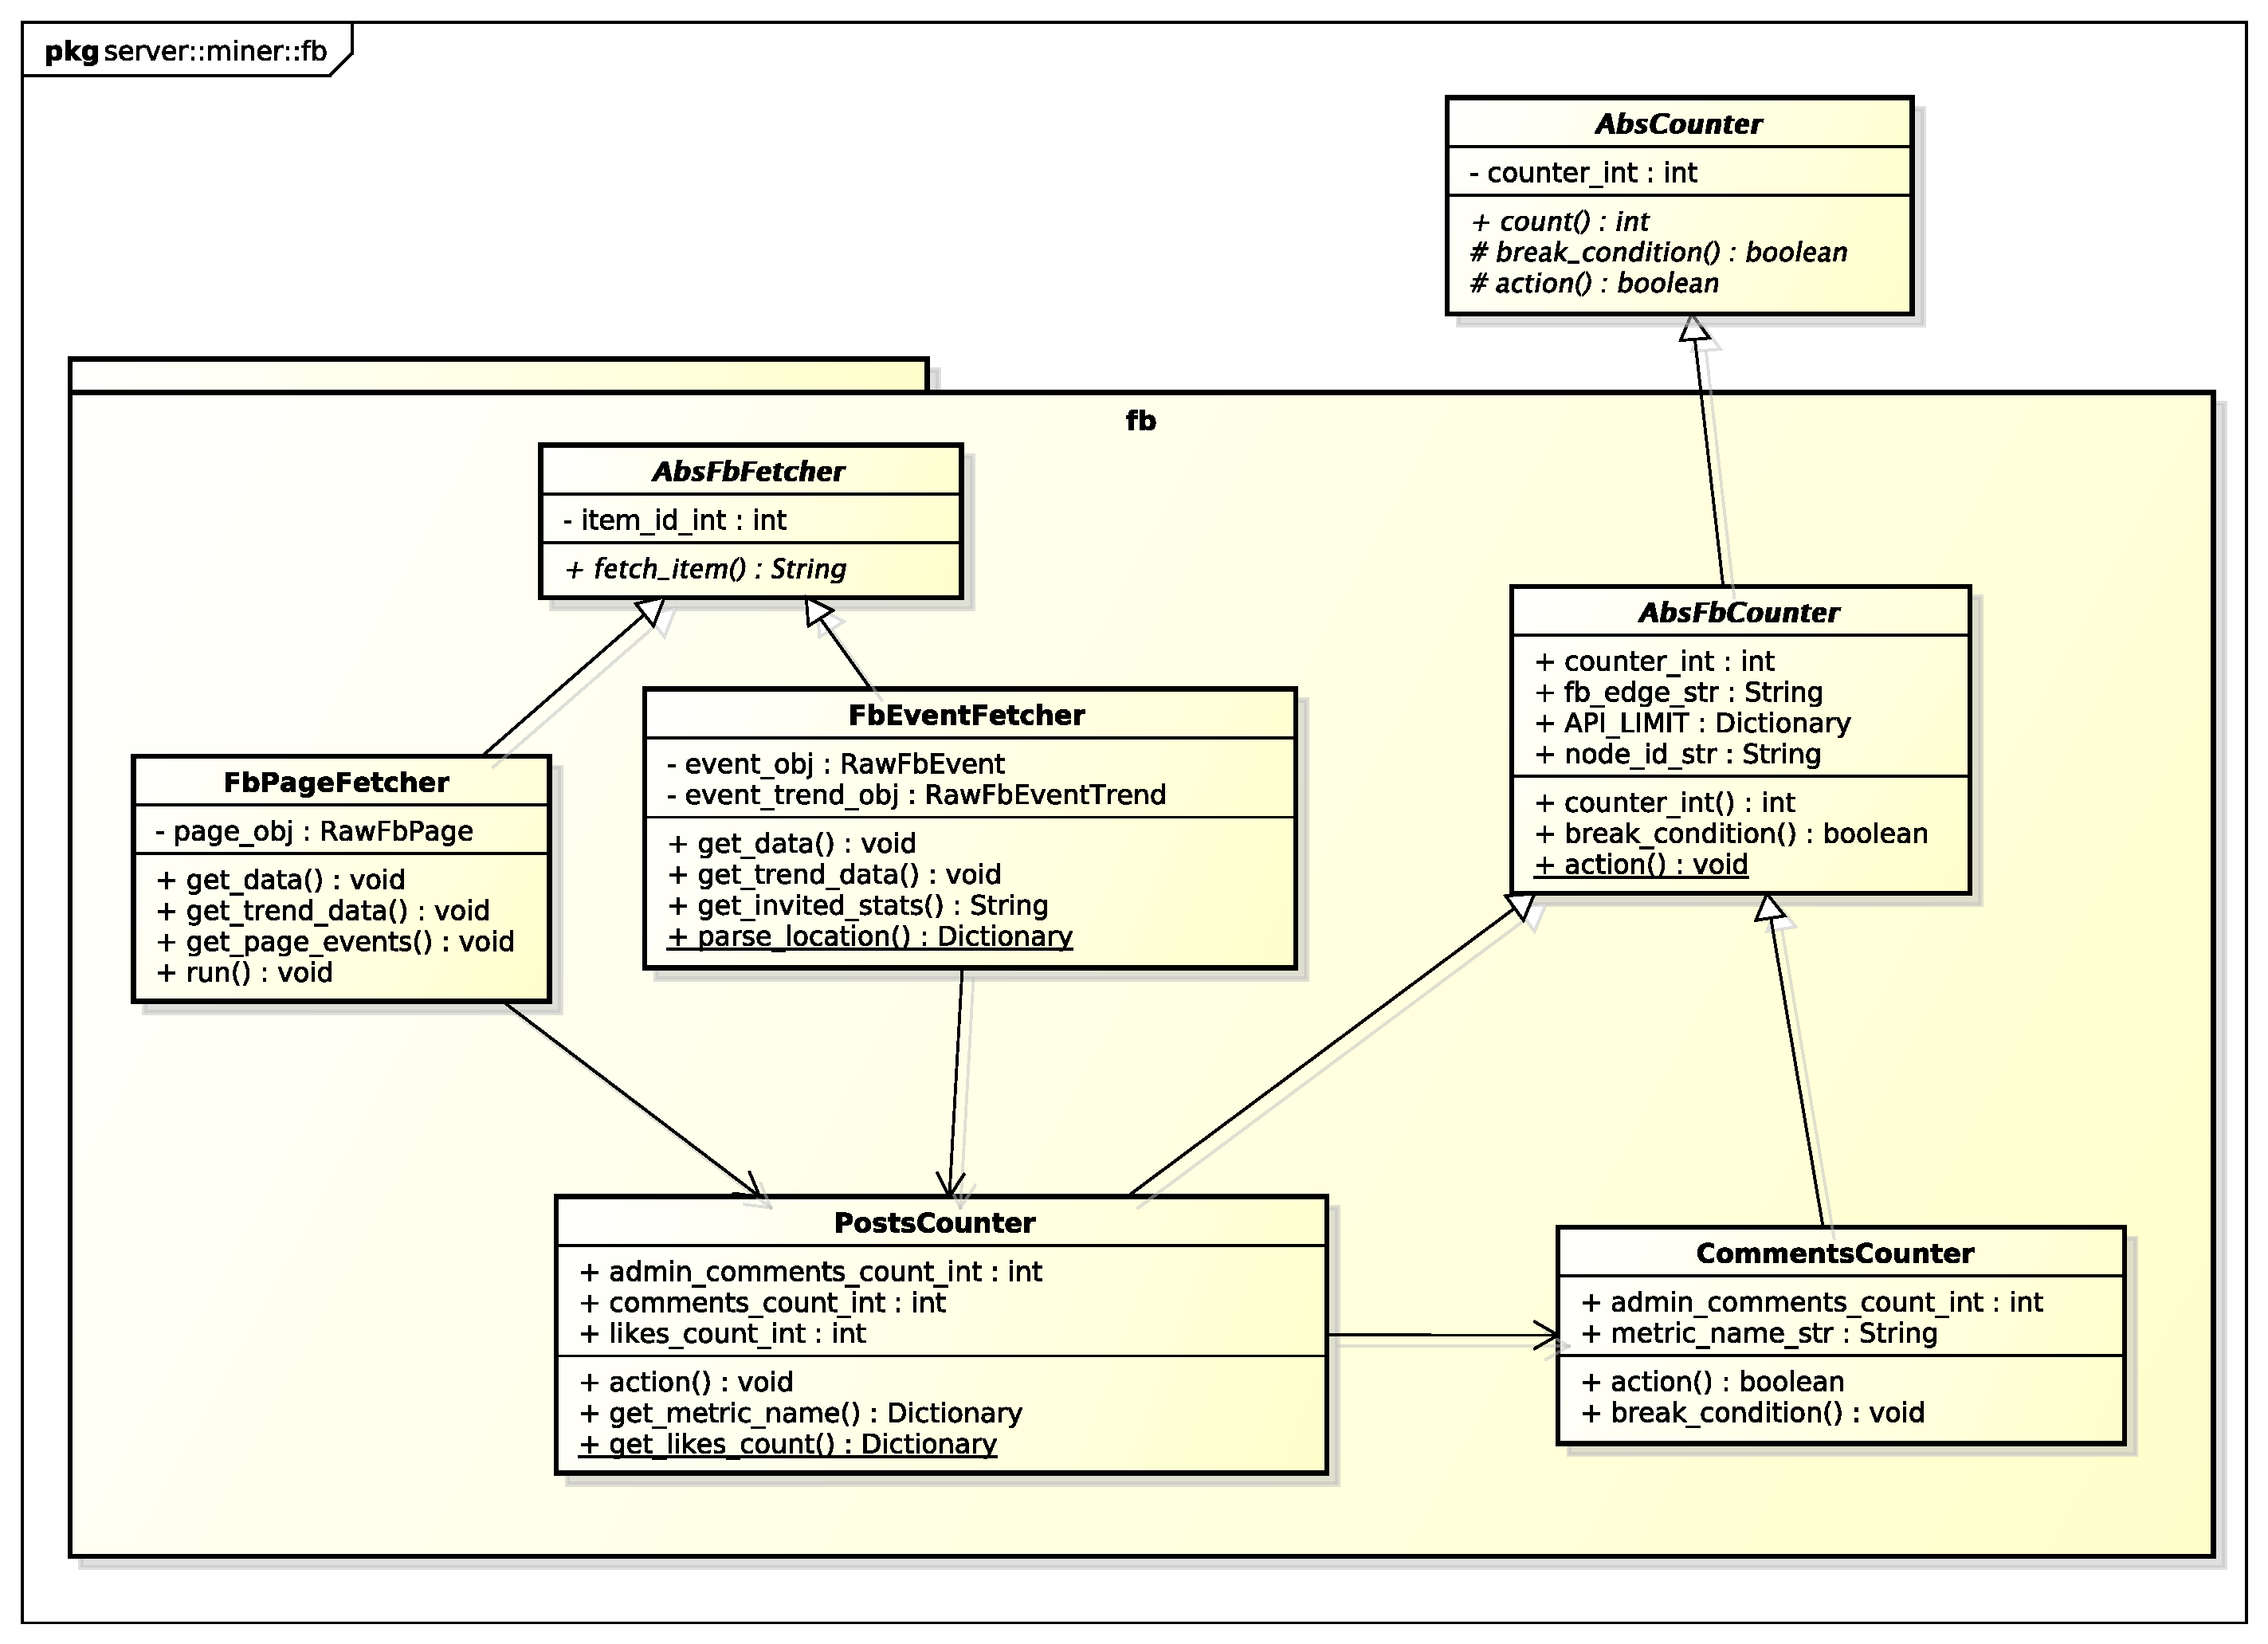
\includegraphics[scale=0.3]{./images/server/miner_fb.pdf}}
	\caption{Package - server::miner::fb}
\end{figure}

\begin{itemize}
  \item \textbf{Descrizione}: è il package che contiene tutte le classi che includono i metodi per prelevare i dati da Facebook e salvarli nel database;
  \item \textbf{Padre}: server::miner
  \item \textbf{Interazione con altri componenti}:
  	\begin{itemize}
  		\item server::db
  	\end{itemize}
\end{itemize}

	\paragraph{Classi} % (fold)
		\subparagraph{server::miner::fb::AbsFbFetcher} % (fold)
		\label{subp:server_miner_fb_AbsFbFetcher}
			\begin{itemize}
				\item \textbf{Descrizione}: classe astratta che rappresenta il padre di ogni fetcher relativo a Facebook;
				\item \textbf{Utilizzo}: contiene un metodo che ricava i dati statici di un'entità Facebook ed un metodo astratto che verrà definito nelle classi figlie;
				\item \textbf{Classi ereditate}: server::miner::AbsFetcher
				\item \textbf{Relazioni con altre classi}:
					\begin{itemize}
						\item server::miner::fb::FbPageFetcher
						\item server::miner::fb::FbEventFetcher
					\end{itemize}
				\item \textbf{Attributi}: 
					\begin{itemize}
						\item \textcolor{forestgreen}{\texttt{+ node\_id\_str : String}}
						\begin{description}
							\item \textbf{Descrizione}: contiene ed identifica l'id univoco della risorsa sul sito Facebook;
						\end{description}
					\end{itemize}
				\item \textbf{Metodi}:   
					\begin{itemize}
						\item \textcolor{forestgreen}{\texttt{+ \_\_init\_\_() : void}}
						\begin{description}
							\item \textbf{Descrizione}: costruttore della classe di default. Inizializza la variabile node\_id\_str con l'id della risorsa;
						\end{description}
						\item \textcolor{forestgreen}{\texttt{+ fetch\_item() : String}}
						\begin{description}
							\item \textbf{Descrizione}: il metodo attiva l'autenticazione sulle API di Facebook ed effettua la chiamata utilizzando node\_id\_str. Ritorna i dati ottenuti dalla chiamata;
						\end{description}
					\end{itemize}
			\end{itemize}
	% subparagraph server_miner_fb_AbsFbFetcher [end]

		\subparagraph{server::miner::fb::FbPageFetcher} % (fold)
		\label{subp:server_miner_fb_FbPageFetcher}
			\begin{itemize}
				\item \textbf{Descrizione}: classe che si occupa ricava i dati dalle pagine Facebook;
				\item \textbf{Utilizzo}: contiene un campo che descrive i dati statici di una pagina, un campo che descrive i dati dinamici ed un metodo che li ricava tramite l'utilizzo della classe \texttt{PostsCounter};
				\item \textbf{Classi ereditate}: server::miner::fb::AbsFbFetcher
				\item \textbf{Relazioni con altre classi}:
					\begin{itemize}
						\item server::miner::fb::PostsCounter
					\end{itemize}
				\item \textbf{Attributi}: 
					\begin{itemize}
						\item \textcolor{forestgreen}{\texttt{+ page\_obj : RawFbPage}}
						\begin{description}
							\item \textbf{Descrizione}: la variabile contiene i risultati della chiamata effettuata tramite le API di Facebook riguardante una pagina utente;
						\end{description}
					\end{itemize}
				\item \textbf{Metodi}:   
					\begin{itemize}
						\item \textcolor{forestgreen}{\texttt{+ \_\_init\_\_(name\_str : String) : void}}
						\begin{description}
							\item \textbf{Descrizione}: costruttore della classe di default. Inizializza la variabile page\_obj ed effettua la costruzione della classe astratta derivata passando l'id della risorsa;
						\end{description}
						\item \textcolor{forestgreen}{\texttt{+ get\_data() : void}}
						\begin{description}
							\item \textbf{Descrizione}: il metodo recupera i dati statici della pagina utente dalle API di Facebook e li memorizza nella base di dati;
						\end{description}
						\item \textcolor{forestgreen}{\texttt{+ get\_trend\_data() : void}}
						\begin{description}
							\item \textbf{Descrizione}: il metodo ha il compito di recuperare tramite le API di Facebook i dati della pagina utente, di rielaborarli e salvarli nella base di dati;
						\end{description}
						\item \textcolor{forestgreen}{\texttt{+ get\_page\_events() : void}}
						\begin{description}
							\item \textbf{Descrizione}: il metodo tramite chiamate alle API di Facebook scarica tutti i dati associati agli eventi di una pagina, li rielabora e li inserisce nella base di dati;
						\end{description}
						\item \textcolor{forestgreen}{\texttt{+ run() : void}}
						\begin{description}
							\item \textbf{Descrizione}: il metodo invoca la costruzione della classe astratta derivata ed avvia l'acquisizione dei dati. Inoltre avvia l'acquisizione dei dati statici e dinamici delle pagine eventi su Facebook;
						\end{description}
					\end{itemize}
			\end{itemize}
		% subparagraph server_miner_fb_FbPageFetcher [end]

		\subparagraph{server::miner::fb::FbEventFetcher} % (fold)
		\label{subp:server_miner_fb_FbEventFetcher}
			\begin{itemize}
				\item \textbf{Descrizione}: classe che ricava i dati di un evento Facebook;
				\item \textbf{Utilizzo}: contiene un campo che descrive i dati statici di un evento, un campo che descrive i dati dinamici e un metodo che li ricava tramite l'utilizzo della classe \texttt{PostsCounter};
				\item \textbf{Classi ereditate}: server::miner::fb::AbsFbFetcher
				\item \textbf{Relazioni con altre classi}:
					\begin{itemize}
						\item server::miner::fb::PostsCounter
					\end{itemize}
				\item \textbf{Attributi}: 
					\begin{itemize}
						\item \item \textcolor{forestgreen}{\texttt{+ parent\_key\_int : int}}
						\begin{description}
							\item \textbf{Descrizione}: viene indicata la chiave del padre per poter collegare il nuovo nodo come figlio;
						\end{description}
						\item \item \textcolor{forestgreen}{\texttt{+ event\_obj : RawFbEvent}}
						\begin{description}
							\item \textbf{Descrizione}: la variabile contiene i risultati della chiamata effettuata tramite le API di Facebook riguardante una pagina evento;
						\end{description}
					\end{itemize}
				\item \textbf{Metodi}:   
					\begin{itemize}
						\item \textcolor{forestgreen}{\texttt{+ \_\_init\_\_() : void}}
						\begin{description}
							\item \textbf{Descrizione}: costruttore della classe di default. Inizializza la classe astratta derivata passandogli l'id della risorsa. Inizializza inoltre event\_obj e parent\_key con i dati a disposizione;
						\end{description}
						\item \textcolor{forestgreen}{\texttt{+ get\_invited\_stats() : Dictionary}}
						\begin{description}
							\item \textbf{Descrizione}: il metodo recupera i dati statici riguardanti le statistiche di partecipazione della pagina evento tramite le API di Facebook e li memorizza nella base di dati;
						\end{description}
						\item \textcolor{forestgreen}{\texttt{+ get\_data() : void}}
						\begin{description}
							\item \textbf{Descrizione}: il metodo recupera i dati statici della pagina evento tramite le API di Facebook e li memorizza nella base di dati;
						\end{description}
						\item \textcolor{forestgreen}{\texttt{+ get\_trend\_data() : void}}
						\begin{description}
							\item \textbf{Descrizione}: il metodo ha il compito di recuperare tramite le API di Facebook i dati della pagina evento, di rielaborarli e salvarli nella base di dati;
						\end{description}
						\item \textcolor{forestgreen}{\texttt{+ static parse\_location(event: String) : Dictionary}}
						\begin{description}
							\item \textbf{Descrizione}: il metodo deve essere dichiarato statico. Tramite l'uso del metodo GeoCodeHelper si ricavano latitudine e longitudine e si restituiscono con tipo dizionario;
						\end{description}
					\end{itemize}
			\end{itemize}
	% subparagraph server_miner_fb_FbEventFetcher [end]

		\subparagraph{server::miner::fb::AbsFbCounter} % (fold)
		\label{subp:server_miner_fb_AbsFbCounter}
			\begin{itemize}
				\item \textbf{Descrizione}: classe astratta che rappresenta il padre per tutte le classi counter delle metriche di Facebook;
				\item \textbf{Utilizzo}: classe che contiene l'id delle metriche su cui effettuare il counting, questa classe effettua l'overloading dei metodi della classe padre specificando la struttura dell'algoritmo per il counting su dati Facebook;
				\item \textbf{Classi ereditate}: server::miner::AbsCounter
				\item \textbf{Relazioni con altre classi}:
					\begin{itemize}
						\item server::miner::fb::PostsCounter
						\item server::miner::fb::CommentsCounter
					\end{itemize}
				\item \textbf{Attributi}:  
					\begin{itemize}
						\item \textcolor{forestgreen}{\texttt{+ API\_LIMIT : Dictionary}}
						\begin{description}
							\item \textbf{Descrizione}: la varibile contiene un dizionario di chiavi-valore, riguardanti i limiti delle chiamate alle API Facebook;
						\end{description}
						\item \textcolor{forestgreen}{\texttt{+ node\_id\_str : String}}
						\begin{description}
							\item \textbf{Descrizione}: la variabile contiene l'id della risorsa univoca presente in Facebook;
						\end{description}
						\item \textcolor{forestgreen}{\texttt{+ fb\_edge\_str : String}}
						\begin{description}
							\item \textbf{Descrizione}: la variabile contiene il parametro richiesto dalle API di Facebook per ricavare i vari tipi di dato associati ad una metrica evento o pagina;
						\end{description}
						\item \textcolor{forestgreen}{\texttt{+ counter\_int : int}}
						\begin{description}
							\item \textbf{Descrizione}: la variabile contiene il numero di occorrenze dell'oggetto specifico di Facebook;
						\end{description}
					\end{itemize}
				\item \textbf{Metodi}:   
					\begin{itemize}
						\item \textcolor{forestgreen}{\texttt{+ \_\_init\_\_(node\_id : int, fb\_edge : String)}}
						\begin{description}
							\item \textbf{Descrizione}: costruttore della classe di default. Il metodo inizializza le variabili passate e inizializza a 0 il counter\_int;
						\end{description}
						\item \textcolor{forestgreen}{\texttt{+ counter\_int() : int}}
						\begin{description}
							\item \textbf{Descrizione}: il metodo conta le occorrenze dell'oggetto Facebook passato dal costruttore;
						\end{description}
						\item \textcolor{forestgreen}{\texttt{+ break\_condition() : boolean}}
						\begin{description}
							\item \textbf{Descrizione}: il metodo definisce le condizioni di arresto del loop per il counting;
						\end{description}
						\item \textcolor{forestgreen}{\texttt{+ abstract action() : void}}
						\begin{description}
							\item \textbf{Descrizione}: il metodo in questa classe viene solamente marcato come astratto, verrà implementato successivamente nelle classi figlie. Il metodo viene utilizzato in ogni elemento ciclato;
						\end{description}
					\end{itemize}
			\end{itemize}
	% subparagraph server_miner_fb_AbsFbCounter [end]


	\subparagraph{server::miner::fb::PostsCounter} % (fold)
		\label{subp:server_miner_fb_PostsCounter}
			\begin{itemize}
				\item \textbf{Descrizione}: classe che descrive l'algoritmo per calcolare il numero dei post per ogni evento o pagina;
				\item \textbf{Utilizzo}: classe che contiene un campo per il numero dei like e un campo per il numero dei talking about per ogni post di Facebook;
				\item \textbf{Classe ereditate}: server::miner::fb::AbsFbCounter
				\item \textbf{Relazioni con altre classi}:
					\begin{itemize}
						\item server::miner::fb::CommentsCounter
					\end{itemize}
				\item \textbf{Attributi}:  
					\begin{itemize}
						\item \textcolor{forestgreen}{\texttt{+ admin\_comments\_count\_int : int}}
						\begin{description}
							\item \textbf{Descrizione}: la variabile contiene il numero di commenti dell'amministratore;
						\end{description}
						\item \textcolor{forestgreen}{\texttt{+ comments\_count\_int : int}}
						\begin{description}
							\item \textbf{Descrizione}: la variabile contiene il numero di commenti totali;
						\end{description}
						\item \textcolor{forestgreen}{\texttt{+ likes\_count\_int : int}}
						\begin{description}
							\item \textbf{Descrizione}: la variabile contiene il numero di likes della pagina;
						\end{description}
					\end{itemize}
				\item \textbf{Metodi}:  
					\begin{itemize}
						\item \textcolor{forestgreen}{\texttt{+ \_\_init\_\_(node\_id\_str : String, fb\_edge\_str : String) : void}}
						\begin{description}
							\item \textbf{Descrizione}: costruttore della classe di default. Il metodo invoca la costruzione della classe astratta derivata settando l'id della risorsa e il tipo di metrica associata. Inoltre inizializza a 0 le variabili per il conteggio;
						\end{description}
						\item \textcolor{forestgreen}{\texttt{+ action() : void}}
						\begin{description}
							\item \textbf{Descrizione}: il metodo viene definito. Effettua la somma dei commenti e dei likes di una pagina Facebook;
						\end{description}
						\item \textcolor{forestgreen}{\texttt{+ get\_metric\_name(): Dictionary}}
						\begin{description}
							\item \textbf{Descrizione}: il metodo identifica il tipo di pagina analizzate e restituisce un dizionario contenente il tipo;
						\end{description}
						\item \textcolor{forestgreen}{\texttt{+ static get\_likes\_count(post\_id : String) : Dictionary}}
						\begin{description}
							\item \textbf{Descrizione}: il metodo in questa classe viene marcato astratto, implementa il conteggio dei like nei post di una pagina Facebook. Ritorna un dizionario con la quantità di likes ottenuti;
						\end{description}
					\end{itemize}
			\end{itemize}
		% subparagraph server_miner_fb_PostsCounter

	\subparagraph{server::miner::fb::CommentsCounter} % (fold)
		\label{subp:server_miner_fb_CommentsCounter}
			\begin{itemize}
				\item \textbf{Descrizione}: classe che descrive l'algoritmo per calcolare il numero di commenti per ogni post;
				\item \textbf{Utilizzo}: classe che ricava il numero di commenti per ogni post;
				\item \textbf{Classe ereditate}: server::miner::fb::AbsFbCounter
				\item \textbf{Attributi}: 
					\begin{itemize}
						\item \textcolor{forestgreen}{\texttt{+ admin\_comments\_count\_int : int}}
						\begin{description}
							\item \textbf{Descrizione}: variabile contenente il numero di commenti effettuati dall'admin della pagina Facebook ;
						\end{description}
						\item \textcolor{forestgreen}{\texttt{+ metric\_name\_str : String}}
						\begin{description}
							\item \textbf{Descrizione}: la variabile contiene il parametro ricavare i vari tipi di dato associati ad una metrica evento o pagina; ;
						\end{description}
					\end{itemize}
				\item \textbf{Metodi}:  
					\begin{itemize}
						\item \textcolor{forestgreen}{\texttt{+ \_\_init\_\_(node\_id\_str : int, metric\_name\_str: String, fb\_edge\_str : String) : void}}
						\begin{description}
							\item \textbf{Descrizione}: costruttore della classe di default. Il metodo invoca il costruttore della classe astratta passandogli l'id della risorsa e il tipo di metrica da applicare alla risorsa. Vengono inoltre inizializzate le variabili a 0;
						\end{description}
						\item \textcolor{forestgreen}{\texttt{+ action() : boolean}}
						\begin{description}
							\item \textbf{Descrizione}: il metodo effettua i conteggi per ricavare la quanità di commenti dell'utente amministratore;
						\end{description}
						\item \textcolor{forestgreen}{\texttt{+ break\_condition() : void}}
						\begin{description}
							\item \textbf{Descrizione}: il metodo viene definito ma non implementato;
						\end{description}
					\end{itemize}
			\end{itemize}
	% subparagraph server_miner_fb_CommentsCounter

\subsubsection{server::miner::tw} % (fold)
\label{ssub:bdsm_app_server_miner_tw}

\begin{itemize}
	\item \textbf{Descrizione}: è il package che contiene tutte le classi che includono i metodi per prelevare i dati da Twitter e salvarli nel database;
	\item \textbf{Padre}: server::miner
	\item \textbf{Interazione con altri componenti}:
		\begin{itemize}
			\item server::db
		\end{itemize}
\end{itemize}

	\begin{figure}[!htbp]
		\centering
		\centerline{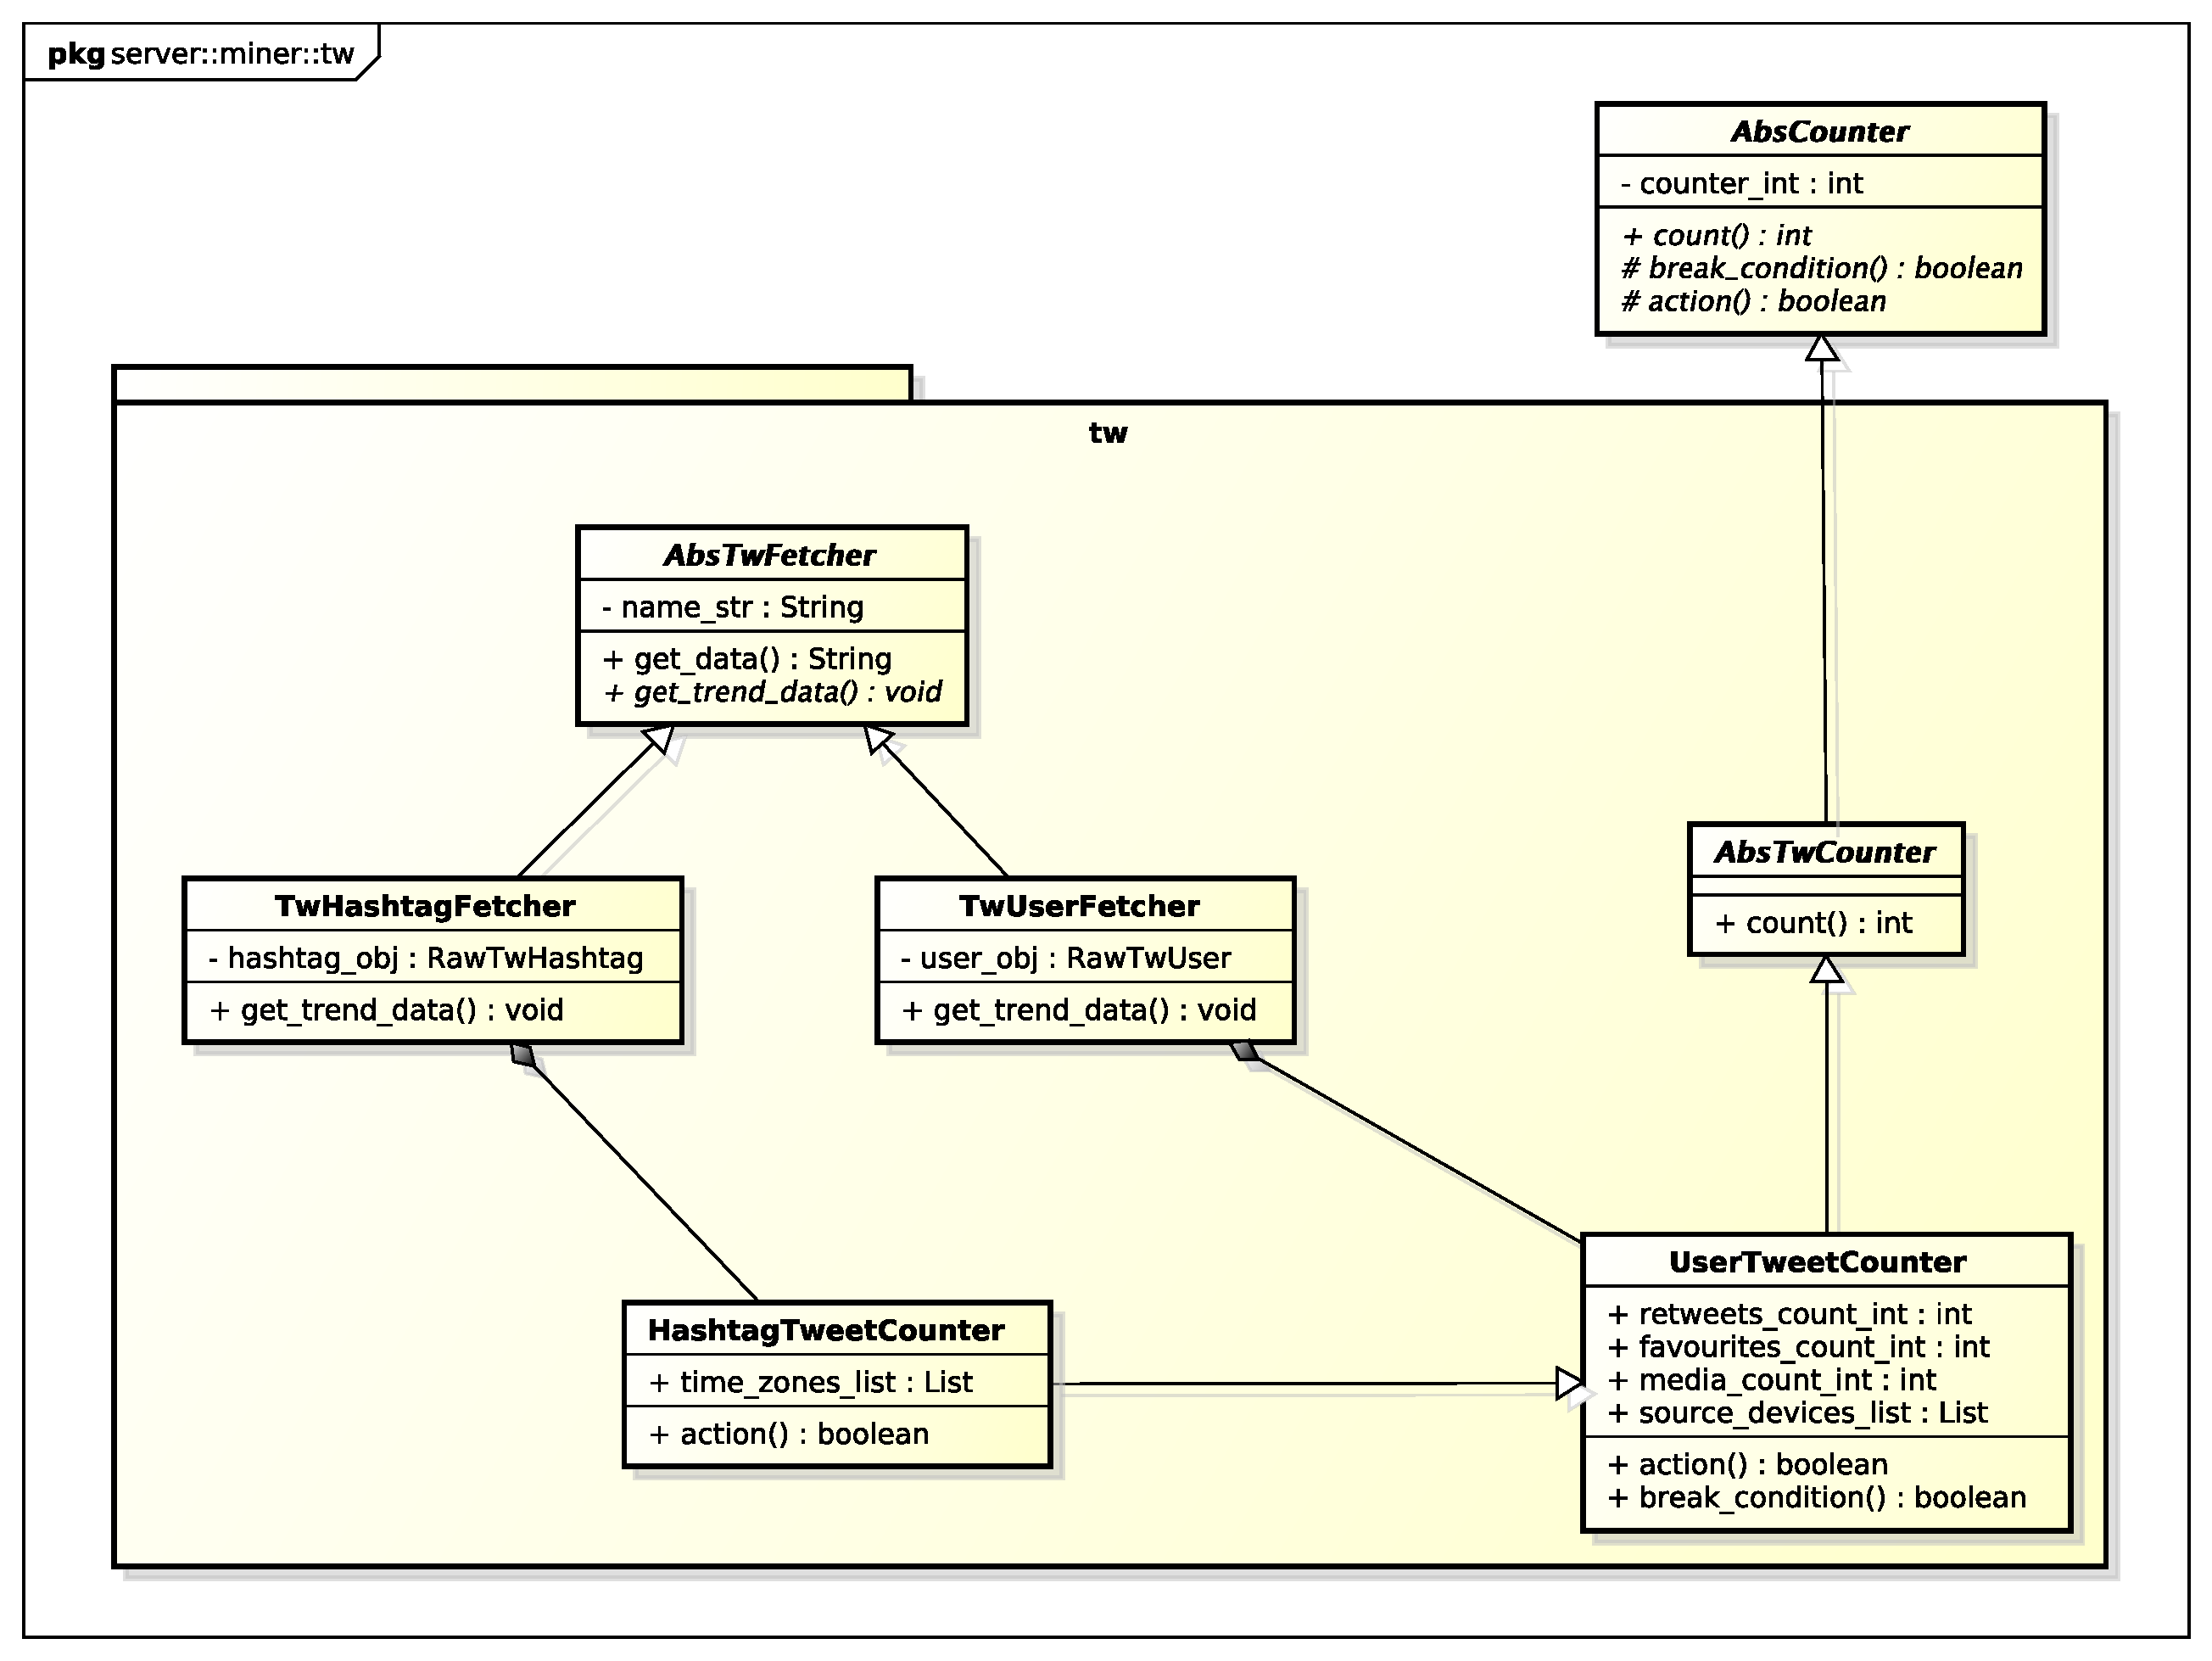
\includegraphics[scale=0.4]{./images/server/miner_tw.pdf}}
		\caption{Package - server::miner::tw}
	\end{figure}

	\paragraph{Classi} % (fold)
	\subparagraph{server::miner::tw::AbsTwFetcher} % (fold)
		\label{subp:server_miner_tw_AbsTwFetcher}
			\begin{itemize}
				\item \textbf{Descrizione}: classe astratta che rappresenta il padre di ogni fetcher relativo a Twitter;
				\item \textbf{Utilizzo}: contiene un metodo che ricava i dati statici di un'entità Twitter ed un metodo astratto che verrà definito nelle classi figlie;
				\item \textbf{Classi ereditate}: server::miner::AbsFetcher
				\item \textbf{Relazioni con altre classi}:
					\begin{itemize}
						\item server::miner::tw::TwHashtagFetcher
						\item server::miner::tw::TwUserFetcher
					\end{itemize}
				\item \textbf{Attributi}:   
					\begin{itemize}
						\item \textcolor{forestgreen}{\texttt{+ name\_str : String}}
						\begin{description}
							\item \textbf{Descrizione}: la variabile contiene l'id univoco della risorsa presente nel social network Twitter;
						\end{description}
					\end{itemize}
				\item \textbf{Metodi}:  
					\begin{itemize}
						\item \textcolor{forestgreen}{\texttt{+ \_\_init\_\_(name\_str : String)}}
						\begin{description}
							\item \textbf{Descrizione}: costruttore della classe di default. Il metodo invoca la classe astratta per la costruzione;
						\end{description}
					\end{itemize}
			\end{itemize}
		% subparagraph server_miner_tw_AbsTwFetcher

	\subparagraph{server::miner::tw::TwHashtagFetcher} % (fold)
		\label{subp:server_miner_tw_TwHashtagFetcher}
			\begin{itemize}
				\item \textbf{Descrizione}: classe che ricava i dati degli hashtag di Twitter;
				\item \textbf{Utilizzo}: classe che contiene un campo che descrive i dati statici di un hashtag di Twitter e un metodo che ricava i dati dinamici tramite l'utilizzo di \texttt{HashtagTweetCounter};
				\item \textbf{Classi ereditate}: server::miner::tw::AbsTwFetcher
				\item \textbf{Relazioni con altre classi}:
					\begin{itemize}
						\item server::miner::tw::HashtagTweetCounter
					\end{itemize}
				\item \textbf{Attributi}:    
					\begin{itemize}
						\item \textcolor{forestgreen}{\texttt{+ hashtag\_obj : RawTwHashtag}}
						\begin{description}
							\item \textbf{Descrizione}: la variabile contiene l'oggetto RawTwHashtag per poterne poi aggiungere i figli associati;
						\end{description}
					\end{itemize}
				\item \textbf{Metodi}:  
					\begin{itemize}
						\item \textcolor{forestgreen}{\texttt{+ \_\_init\_\_(name\_str : String)}}
						\begin{description}
							\item \textbf{Descrizione}: costruttore della classe di default. Il metodo invoca la classe astratta per la costruzione passando il nome della risorsa. Istanzia l'oggetto hashtag\_obj;
						\end{description}
						\item \textcolor{forestgreen}{\texttt{+ get\_data() : void}}
						\begin{description}
							\item \textbf{Descrizione}: il metodo costruisce, se non già presente, l'oggetto padre contenente il nome e la data di creazione della risorsa ricercata;
						\end{description}
						\item \textcolor{forestgreen}{\texttt{+ get\_trend\_data() : void}}
						\begin{description}
							\item \textbf{Descrizione}: il metodo ha il compito di ricercare i dati di trend per l'hashtag. Dopo averli sommati, vengono immagazzinati nella base di dati;
						\end{description}
					\end{itemize}
			\end{itemize}
		% subparagraph server_miner_tw_TwHashtagFetcher

	\subparagraph{server::miner::tw::TwUserFetcher} % (fold)
		\label{subp:server_miner_tw_TwUserFetcher}
			\begin{itemize}
				\item \textbf{Descrizione}: classe che ricava i dati degli utenti di Twitter;
				\item \textbf{Utilizzo}: classe che contiene un campo che descrive i dati statici dell'utente ed un metodo che ricava i dati dinamici tramite l'utilizzo di \texttt{UserTweetCounter};
				\item \textbf{Classi ereditate}: server::miner::tw::AbsTwFetcher
				\item \textbf{Relazioni con altre classi}:
					\begin{itemize}
						\item server::miner::tw::UserTweetCounter
					\end{itemize}
				\item \textbf{Attributi}:    
					\begin{itemize}
						\item \textcolor{forestgreen}{\texttt{+ user\_obj : RawTwUser}}
						\begin{description}
							\item \textbf{Descrizione}: la variabile contiene l'oggetto RawTwUser per poterne poi aggiungere i figli associati;
						\end{description}
					\end{itemize}
				\item \textbf{Metodi}:  
					\begin{itemize}
						\item \textcolor{forestgreen}{\texttt{+ \_\_init\_\_(name\_str: String) : void}}
						\begin{description}
							\item \textbf{Descrizione}: costruttore della classe di default. Il metodo invoca la classe astratta per la costruzione passando il nome della risorsa. Istanzia l'oggetto user\_obj;
						\end{description}
						\item \textcolor{forestgreen}{\texttt{+ get\_data() : void}}
						\begin{description}
							\item \textbf{Descrizione}: il metodo tramite le API di Twitter ottiene i dati statici della pagina utente e li memorizza nella base di dati;
						\end{description}
						\item \textcolor{forestgreen}{\texttt{+ get\_trend\_data() : void}}
						\begin{description}
							\item \textbf{Descrizione}: il metodo tramite le API di Twitter ottiene i dati dinamici della pagina utente e tramite ulteriori chiamate ai metodi ne ricava i dati di trend. Alla fine della elaborazione viene creato l'oggetto padre ed i relativi figli;
						\end{description}
					\end{itemize}
			\end{itemize}
		% subparagraph server_miner_tw_TwUserFetcher

	\subparagraph{server::miner::tw::AbsTwCounter} % (fold)
		\label{subp:server_miner_tw_AbsTwCounter}
			\begin{itemize}
				\item \textbf{Descrizione}: classe astratta che rappresenta il padre per tutte le classi counter delle metriche di Twitter;
				\item \textbf{Utilizzo}: oltre a contenere l’id delle metriche su cui effettuare il counting, questa classe effettua l'overloading dei metodi della classe padre specificando la struttura dell'algoritmo per il counting su dati Twitter;
				\item \textbf{Classi ereditate}: server::miner::AbsCounter
				\item \textbf{Relazioni con altre classi}:
					\begin{itemize}
						\item server::miner::UserTweetCounter
					\end{itemize}
				\item \textbf{Attributi}:
					\begin{itemize}
						\item \textcolor{forestgreen}{\texttt{+ recent\_tweet : String}}
						\begin{description}
							\item \textbf{Descrizione}: la variabile contiene il nome della metrica rispetto alla pagina Twitter analizzata;
						\end{description}
					\end{itemize}
				\item \textbf{Metodi}: 
					\begin{itemize}
						\item \textcolor{forestgreen}{\texttt{+ \_\_init\_\_(recent\_tweet : String) : void}}
						\begin{description}
							\item \textbf{Descrizione}: costruttore della classe di default. Il metodo invoca la classe astratta per la costruzione passando la metrica della risorsa. Istanzia l'oggetto recent\_tweet;
						\end{description}
						\item \textcolor{forestgreen}{\texttt{+ count() : Boolean}}
						\begin{description}
							\item \textbf{Descrizione}: il metodo conta le occorrenze dell'oggetto passato implementando l'azione si stop quando necessario. Ritorna False quando l'azione non è più necessaria;
						\end{description}
						\item \textcolor{forestgreen}{\texttt{+ abstract action() : void}}
						\begin{description}
							\item \textbf{Descrizione}: il metodo viene definito astratto ma non viene implementato;
						\end{description}
						\item \textcolor{forestgreen}{\texttt{+ abstract break\_condition() : void}}
						\begin{description}
							\item \textbf{Descrizione}: il metodo viene definito astratto ma non viene implementato;
						\end{description}
					\end{itemize}
			\end{itemize}
		% subparagraph server_miner_tw_AbsTwCounter

	\subparagraph{server::miner::tw::UserTweetCounter} % (fold)
		\label{subp:server_miner_tw_UserTweetCounter}
			\begin{itemize}
				\item \textbf{Descrizione}: classe che descrive l'algoritmo per il counting dei campi di un tweet, relativo ad un utente, di cui ci interessa fare un trend;
				\item \textbf{Utilizzo}: classe che ricava il numero dei retweets, il numero dei favoriti, il tipo di device, e il numero di media per ogni tweet;
				\item \textbf{Classi ereditate}: server::miner::tw::AbsTwCounter
				\item \textbf{Attributi}:    
					\begin{itemize}
						\item \textcolor{forestgreen}{\texttt{+ favourites\_count\_int : int}}
						\begin{description}
							\item \textbf{Descrizione}: la variabile contiene il numero di favoriti contati nei tweets;
						\end{description}
						\item \textcolor{forestgreen}{\texttt{+ retweets\_count\_int : int}}
						\begin{description}
							\item \textbf{Descrizione}: la variabile contiene il numero retweets contati nei tweets;
						\end{description}
						\item \textcolor{forestgreen}{\texttt{+ source\_devices\_list : List}}
						\begin{description}
							\item \textbf{Descrizione}: la variabile contiene una lista chiave-valore di dispositivi e quantità utilizzati per la pubblicazione dei tweets;
						\end{description}
						\item \textcolor{forestgreen}{\texttt{+ date\_created\_date : Date}}
						\begin{description}
							\item \textbf{Descrizione}: la variabile contiene la data di acquisizione dei dati;
						\end{description}
					\end{itemize}
				\item \textbf{Metodi}:  
					\begin{itemize}
						\item \textcolor{forestgreen}{\texttt{+ \_\_init\_\_(name\_str : String) : void}}
						\begin{description}
							\item \textbf{Descrizione}: costruttore della classe di default. Il metodo invoca la classe astratta per la costruzione passando l'id della risorsa. Istanzia i contatori a 0 e la lista vuota;
						\end{description}
						\item \textcolor{forestgreen}{\texttt{+ action(tweet : TweetUserFetcher) : void}}
						\begin{description}
							\item \textbf{Descrizione}: il metodo invoca la somma dei campi dati dell'oggetto passato;
						\end{description}
						\item \textcolor{forestgreen}{\texttt{+ break\_condition(data : Date) : Boolean}}
						\begin{description}
							\item \textbf{Descrizione}: il metodo definisce la condizione di stop per i cicli di somma;
						\end{description}
					\end{itemize}
			\end{itemize}
		% subparagraph server_miner_tw_UserTweetCounter


	\subparagraph{server::miner::tw::HashtagTweetCounter} % (fold)
		\label{subp:server_miner_tw_HashtagTweetCounter}
			\begin{itemize}
				\item \textbf{Descrizione}: classe che descrive l'algoritmo per il counting dei campi di un tweet, relativo ad un hashtag, di cui ci interessa fare un trend;
				\item \textbf{Utilizzo}: classe che ricava anche la time zone di ogni tweet;
				\item \textbf{Classi ereditate}: server::miner::tw::UserTweetCounter
				\item \textbf{Attributi}:    
					\begin{itemize}
						\item \textcolor{forestgreen}{\texttt{+ favourites\_count\_int : int}}
						\begin{description}
							\item \textbf{Descrizione}: la variabile contiene la somma dei favoriti dell'hashtag Twitter;
						\end{description}
						\item \textcolor{forestgreen}{\texttt{+ retweets\_count\_int : int}}
						\begin{description}
							\item \textbf{Descrizione}: la variabile contiene la somma dei retweets dell'hashtag Twitter;
						\end{description}
						\item \textcolor{forestgreen}{\texttt{+ source\_devices\_list : List}}
						\begin{description}
							\item \textbf{Descrizione}: la variabile contiene la lista formata da chiave-valore dei dispositivi utilizzati per la scrittura dell'hashtag Twitter;
						\end{description}
						\item \textcolor{forestgreen}{\texttt{+ date\_created\_date : Date}}
						\begin{description}
							\item \textbf{Descrizione}: la variabile contiene la data di acquisizione dei dati;
						\end{description}
						\item \textcolor{forestgreen}{\texttt{+ time\_zone\_list : Date}}
						\begin{description}
							\item \textbf{Descrizione}: la variabile contiene la lista formata da chiave-valore dei timezone della pubblicazione dell'hashtag Twitter;
						\end{description}
						\item \textcolor{forestgreen}{\texttt{+ tweets\_count\_int : int}}
						\begin{description}
							\item \textbf{Descrizione}: la variabile contiene la somma dei tweets dell'hashtag Twitter;
						\end{description}
					\end{itemize}
				\item \textbf{Metodi}:  
					\begin{itemize}
						\item \textcolor{forestgreen}{\texttt{+ \_\_init\_\_(name\_str: String) : void}}
						\begin{description}
							\item \textbf{Descrizione}: costruttore della classe di default. Il metodo invoca la classe astratta per la costruzione passando l'id della risorsa. Istanzia i contatori a 0, la lista vuota e la data di creazione;
						\end{description}
						\item \textcolor{forestgreen}{\texttt{+ action(tweet : TwHashtagFetcher) : void}}
						\begin{description}
							\item \textbf{Descrizione}: il metodo definisce i campi dati da sommare;
						\end{description}
					\end{itemize}
			\end{itemize}
		% subparagraph server_miner_tw_HashtagTweetCounter



\subsubsection{server::miner::ig} % (fold)
\label{ssub:bdsm_app_server_miner_ig}
\begin{figure}[htbp]
	\centering
	\centerline{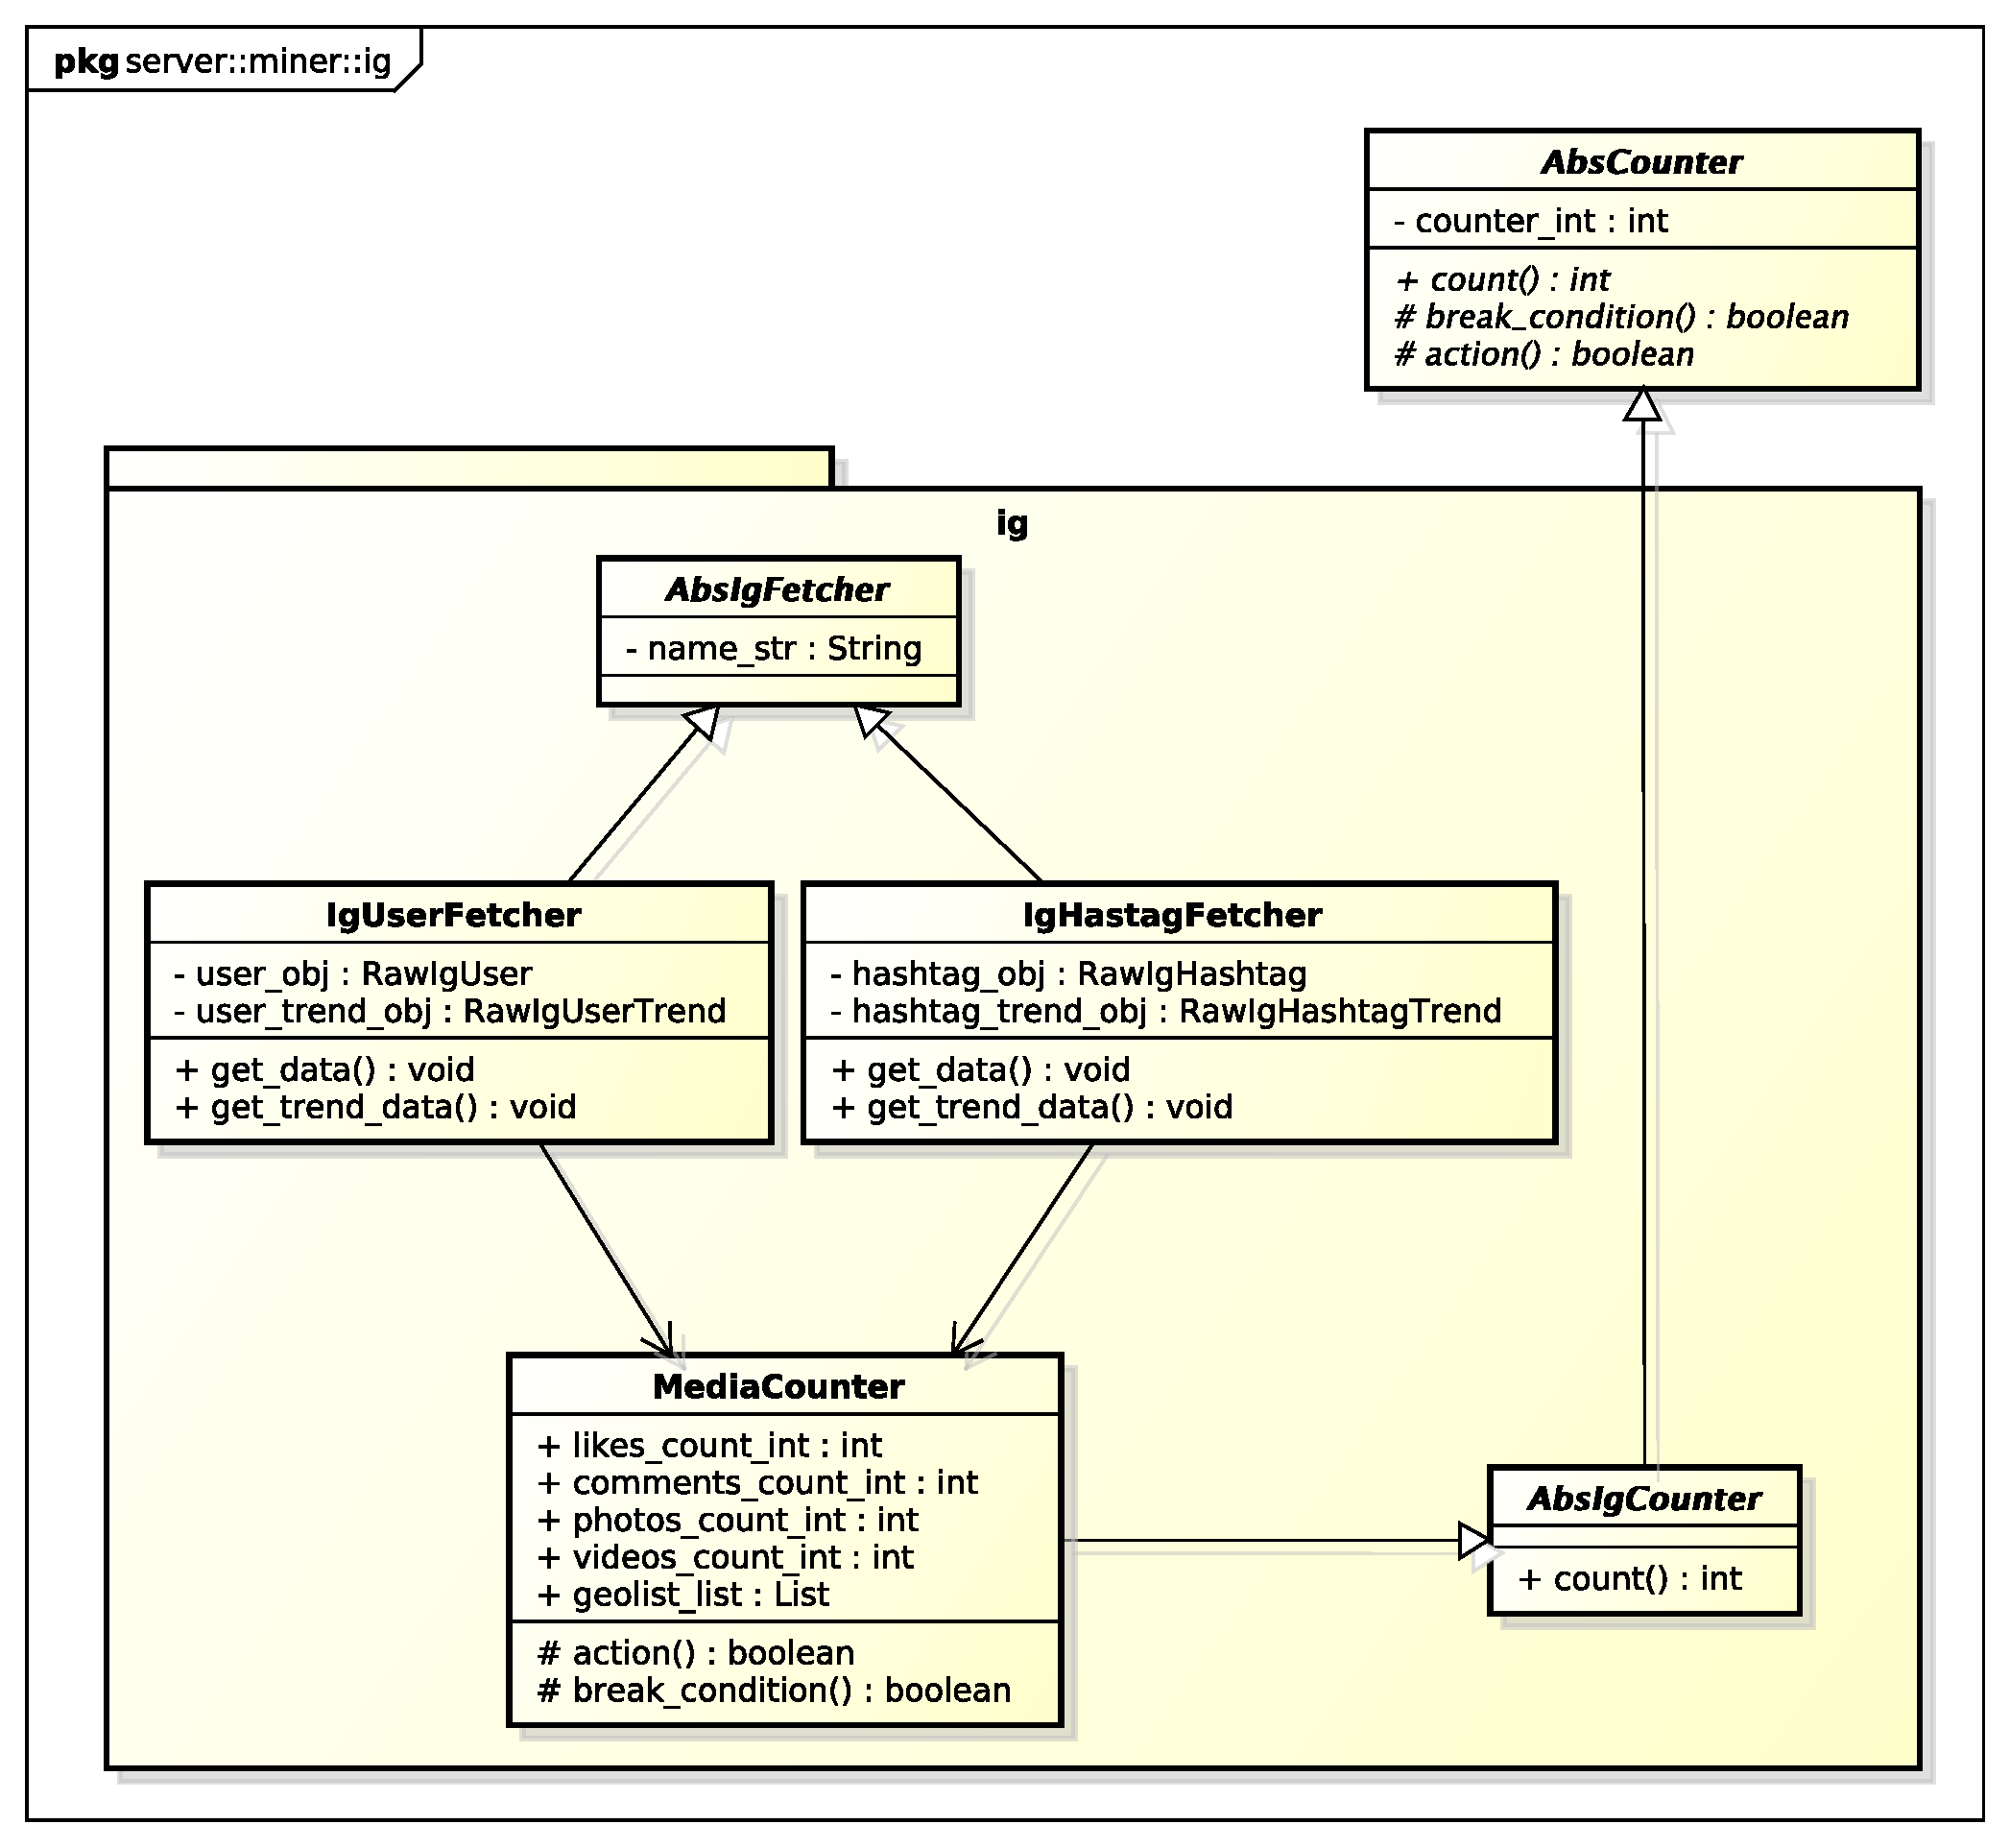
\includegraphics[scale=0.4]{./images/server/miner_ig.pdf}}
	\caption{Package - server::miner::ig}
\end{figure}


\begin{itemize}
  \item \textbf{Descrizione}: è il package che contiene tutte le classi che includono i metodi per prelevare i dati da Instagram e salvarli nel database;
  \item \textbf{Padre}: server::miner
   \item \textbf{Interazione con altri componenti}:
  	\begin{itemize}
  		\item server::db
  	\end{itemize}
\end{itemize}

	\paragraph{Classi} % (fold)
	\subparagraph{server::miner::ig::AbsIgFetcher} % (fold)
		\label{subp:server_miner_ig_AbsIgFetcher}
			\begin{itemize}
				\item \textbf{Descrizione}: classe astratta che rappresenta il padre di ogni fetcher relativo a Instagram;
				\item \textbf{Utilizzo}: contiene un metodo che ricava i dati statici di un'entità Instagram ed un metodo astratto che verrà definito nelle classi figlie;
				\item \textbf{Classi ereditate}: server::miner::AbsFetcher
				\item \textbf{Relazioni con altre classi}:
					\begin{itemize}
						\item server::miner::ig::IgUserFetcher
						\item server::miner::ig::IgHashtagFetcher
					\end{itemize}
				\item \textbf{Attributi}:    
					\begin{itemize}
						\item name\_str : String
					\end{itemize}
				\item \textbf{Metodi}:  
					\begin{itemize}
						\item public get\_data() : void
						\item public get\_trend\_data() : void
					\end{itemize}
			\end{itemize}
		% subparagraph server_miner_ig_AbsIgFetcher

	\subparagraph{server::miner::ig::IgUserFetcher} % (fold)
		\label{subp:server_miner_ig_IgUserFetcher}
			\begin{itemize}
				\item \textbf{Descrizione}: classe che ricava i dati dagli utenti di Instagram;
				\item \textbf{Utilizzo}: classe che contiene un campo che descrive i dati statici dell'utente ed un metodo che ricava i dati dinamici tramite l'utilizzo di \texttt{MediaCounter};
				\item \textbf{Classi ereditate}: server::miner::ig::AbsIgFetcher
				\item \textbf{Relazioni con altre classi}:
					\begin{itemize}
						\item server::miner::ig::MediaCounter
					\end{itemize}
				\item \textbf{Attributi}:    
					\begin{itemize}
						\item user\_obj : RawIgUser
						\item user\_trend\_obj : RawIgUserTrend
					\end{itemize}
				\item \textbf{Metodi}:  
					\begin{itemize}
						\item public get\_data() : void
						\item public get\_trend\_data() : void
					\end{itemize}
			\end{itemize}
		% subparagraph server_miner_ig_IgUserFetcher

	\subparagraph{server::miner::ig::IgHashtagFetcher} % (fold)
		\label{subp:server_miner_ig_IgHashtagFetcher}
			\begin{itemize}
				\item \textbf{Descrizione}: classe che ricava i dati dagli hashtag di Instagram;
				\item \textbf{Utilizzo}: classe che contiene un campo che descrive i dati statici dell'hashtag ed un metodo che ricava i dati dinamici tramite l'utilizzo di \texttt{MediaCounter};
				\item \textbf{Classi ereditate}: server::miner::ig::AbsIgFetcher
				\item \textbf{Relazioni con altre classi}:
					\begin{itemize}
						\item server::miner::ig::MediaCounter
					\end{itemize}
				\item \textbf{Attributi}:    
					\begin{itemize}
						\item hashtag\_obj : RawIgHashtag
						\item hashtag\_trend\_obj : RawIgHashtagTrend
					\end{itemize}
				\item \textbf{Metodi}:  
					\begin{itemize}
						\item public get\_data() : void
						\item public get\_trend\_data() : void
					\end{itemize}
			\end{itemize}
		% subparagraph server_miner_ig_IgHashtagFetcher

	\subparagraph{server::miner::ig::AbsIgCounter} % (fold)
		\label{subp:server_miner_ig_AbsIgCounter}
			\begin{itemize}
				\item \textbf{Descrizione}: classe astratta che rappresenta il padre per tutte le classi counter delle metriche relative ad Instagram;
				\item \textbf{Utilizzo}: classe che contiene l’id delle metriche su cui effettuare il counting, questa classe effettua l'overloading dei metodi della classe padre per specificarne l’utilizzo sui dati relativi ad Instagram;
				\item \textbf{Classi ereditate}: server::miner::AbsCounter
				\item \textbf{Relazioni con altre classi}:
					\begin{itemize}
						\item server::miner::ig::MediaCounter
					\end{itemize}
				\item \textbf{Attributi}: N/A
				\item \textbf{Metodi}: 
					\begin{itemize}
						\item public count() : int
					\end{itemize}
			\end{itemize}
		% subparagraph server_miner_ig_AbsIgCounter


	\subparagraph{server::miner::ig::MediaCounter} % (fold)
		\label{subp:server_miner_ig_MediaCounter}
			\begin{itemize}
				\item \textbf{Descrizione}: classe che descrive l'algoritmo per il counting delle metriche necessarie a descrivere il trend dei media di un utente o di un hashtag  Instagram;
				\item \textbf{Utilizzo}: classe che ricava il numero di commenti, il numero di like, il numero di foto e il numero di video di un media;
				\item \textbf{Classi ereditate}: server::miner::ig::AbsIgCounter
				\item \textbf{Attributi}:    
					\begin{itemize}
						\item public likes\_count\_int : int
						\item public comments\_count\_int : int
						\item public photos\_count\_int : int
						\item public videos\_count\_int : int
						\item public geolist\_list : List
					\end{itemize}
				\item \textbf{Metodi}:  
					\begin{itemize}
						\item protected action() : boolean
						\item protected break\_condition() : boolean
					\end{itemize}
			\end{itemize}
		% subparagraph server_miner_ig_MediaCounter


% subsubsection
